\chapter{The semantics of first-order logic}

We are now ready to tackle the semantics of first-order logic. In some sense, the semantics of first-order logic is very much like the semantics of zeroth-order logic, with the exception of the newly introduced variables and the quantifiers that bind them. On the other hand, the \textit{expressive power} of the language $\mathcal{L}_1$ is vastly more powerful than that of $\mathcal{L}_0$. Indeed, for some, first-order classical logic is \textit{the} logical system, or at any rate, the \textit{strongest but still well-behaved} logical system. At any rate, this added expressive power comes with added complexity, and everything starts with dealing with the semantic values of our variables. 

\section{On the values of variables}

For a moment, let's forget about our logics and consider everyday mathematical practice. Suppose you have a simple equation of one unknown variable as follows: 
\[
(2\times x)+7=57
\]
If you `solve' this equation, you get that $x=25$. Now really, all this means is that if you take the \textit{value of the variable} $x$ to be $25$, then $(2\times x)+7=57$ will come out correct, while if you take \textit{the value of the variable} $x$ to be anything else, it will come out incorrect. Thus, one way we can talk about variables is to assign them a value and see whether the resulting formula is correct, computing with the value assigned. In such cases, the variables function like \textit{temporary constants}. Essentially, what we are saying above is that for a moment, you should understand $(2\times x)+7=57$ the same way as you would understand $(2 \times 25) + 7= 57$. Of course, unlike with constants, what the value of $x$ is is temporarily assigned. For example, in $(5 \times x)+7=107$, the formula will now come out true provided $x$ is assigned the value $20$, not $25$. Clearly, the value of $20$ and $25$ did not change from one equation to the other, but the assigned value of $x$ did, provided the aim is to make the formula correct. And of course, we can assign a value to $x$ that makes neither of these equations come out correct. For example, if $x$ is assigned the value $97$, both equations will come out incorrect. As we shall see presently, our semantics for first-order logic will be founded on these temporary assignments of values to the variables of the language $\mathcal{L}_1$.

Ultimately, our goal is to assign meaning to quantified formulas with no free variables, i.e., quantified closed formulas, in a systematic way. This will be based on a generalization of the idea of temporary assignments of values. For example, take the claim:
\begin{center}
	The equation $(2\times x)+7=57$ has a solution. 
\end{center}
What this means is that \textit{there is} a temporary assignment of a value to the variable $x$ such that $(2\times x)+7=57$ comes out correct. This is clearly a use of the existential quantifier. And clearly, this is true if there really is such an assignment. Moreover, as demonstrated, there is such an assignment (assigning $25$ to $x$), so it is true that the equation has a solution. 

On the other hand, take the claim: 
\begin{center}
	The equation $(0\times x)+7=57$ has a solution. 
\end{center}
This is false, and the reason why it is false is because \textit{there is no} assignment of a value to the variable $x$ such that $(0\times x)+7=57$. 

The same type of reasoning holds for the universal quantifier. For example, for the equation $2 \times (x + 2)=(2 \times x) + 4$, \textit{every} temporary assignment of a value to the variable $x$ makes the equation come out correct. Incidentally, this is equivalent to the fact that \textit{there is no} assignment of a value to the variable $x$ which would make the equation come out incorrect. 

\section{The meaning of terms}

As specified above, the terms of $\mathcal{L}_1$ are the constants and variables of $\mathcal{L}_1$. For $\mathcal{L}_0$, assigning a semantic value to any constant was done through the interpretation function of the structure $\mathbf{S}=\oset{\mathbf{D}, I}$. This will be retained, so that the value of a constant $\cons{n}$ ($n \in \mathbb{N}$) relative to the structure $\mathbf{S}$, in other words (symbols), $I(\cons{n})$, is just some member of $\mathbf{D}$. But again, though variables have a function similar to constants, their semantic value is only temporarily assigned, and is otherwise \textit{variable}. Accordingly, we do not use the interpretation function $I$ to assign values to our variables, but a separate function $\mathbf{a}$ called a \textit{variable assignment}. 

The variable assignment function $\mathbf{a}$ assigns to each \textit{variable} $\var{n}$ ($n \in \mathbb{N}$) a member of $\mathbf{D}$, like $I$ does for constants. But unlike with $I$, we will introduce a device that will allow us to change the variable assignment \textit{inside} a structure $\mathbf{S}$. The basis of this is what is called an $x$-variant assignment $\mathbf{a}'$ for an existing assignment $\mathbf{a}$. Unsurprisingly, $\mathbf{a}'$ is called an $x$-variant assignment of $\mathbf{a}$ because it differs from it in at most what it assigns to the variable $x$. (It should be noted that in usual mathematical fashion, $\mathbf{a}$ may be its own (trivial) $x$-variant assignment, in which case nothing is changed from the initial assignment.) 

Let's look at an example for this. Suppose you have a mathematical statement as follows:
\[
x \times 4 < 2 \times y
\]
Here, we have multiple variables, so each assignment of values to the variables will assign a value to $x$, and to $y$. Suppose we assign the value $5$ to $x$ and $10$ to $y$. This will result in an incorrect statement, since $20<20$ is incorrect. So now take the $x$-variant assignment that assigns $4$ to $x$, but otherwise leaves the assignment as it was. This time, we get a correct statement, since $16 <20$. Of course, we can also take a $y$-variant assignment. And in general, not all $x$- or $y$-variant assignment will make the statement correct. For example, the $y$-variant assignment (to the initial one) where $y=5$ will clearly make it incorrect again. 

We can make the above ideas more precise as follows:

\begin{defn}[Variable assignment]
Given a structure $\mathbf{S}=\oset{\mathbf{D}, I}$, the function $\mathbf{a}: \textsf{VAR}_{\mathcal{L}_1} \to \mathbf{D}$ is a \textit{variable assignment} in $\mathbf{D}$. If $\mathbf{a}'$ is a variable assignment in $\mathbf{D}$ just like $\mathbf{a}$, except possibly for some $x$, $\mathbf{a}'(x)\neq \mathbf{a}(x)$, we call $\mathbf{a}'$ an $x$-variant variable assignment of $\mathbf{a}$. If $\mathbf{a}'(x)=d$ ($d \in D$), i.e., $\mathbf{a}'$ is the $x$-variant variable assignment of $\mathbf{a}$ such that $x$ is sent to $d$ by $\mathbf{a}'$, we may also write $\mathbf{a}^x_d$.
\end{defn}

Let's return to the general picture. Since some terms of the language $\mathcal{L}_1$ are variables, it won't be enough to work solely with the interpretation function $I$ to assign semantic values to our terms in $\mathcal{L}_1$ -- we need a variable assignment too. Clearly, since these terms then go into forming atomic and complex formulas, we will need to relativize the semantic values of expressions of $\mathcal{L}_1$ both to a particular structure $\mathbf{S}=\oset{\mathbf{D}, I}$ and to a corresponding variable assignment $\mathbf{a}$ in $\mathbf{D}$ at any one time. We will introduce some new notation for this. In particular, if $X$ is any expression of $\mathcal{L}_1$, then its semantic value relative to a structure $\mathbf{S}=\oset{\mathbf{D}, I}$ \textit{and} variable assignment $\mathbf{a}$ in $\mathbf{D}$ will be denoted:
\[
I(X)[\mathbf{a}]
\]
Using this notation, we can easily specify what it means to assign a semantic value to a \textit{term} of $\mathcal{L}_1$ as follows:
\begin{defn}[Term values]
Let $\mathbf{S}=\oset{\mathbf{D}, I}$ be any ordered pair such that $\mathbf{D}$ is a non-empty set and $I$ is defined for each $c \in \mathsf{CONS}_{\mathcal{L}_1}$ so that $I(c) \in \mathbf{D}$. Let $\mathbf{a}$ be a variable assignment in $\mathbf{D}$ as above. Then, for each term $t \in \mathsf{TERM}_{\mathcal{L}_1}$, we define the value of $t$ in the structure $\mathbf{S}$ relative to the variable assignment $\mathbf{a}$ as follows:
\begin{enumerate}
	\item if $t=x$ for some $x \in \textsf{VAR}_{\mathcal{L}_1}$, $I(t)[\mathbf{a}]=\mathbf{a}(t)$;
	\item if $t=c$ for some $c \in \textsf{CONS}_{\mathcal{L}_1}$, $I(t)[\mathbf{a}]=I(c)$.
\end{enumerate}
\end{defn}

\begin{remark}
Take some time to try and thoroughly understand the above definition. What it says is that if a term is a variable, then its value is taken care of by the variable assignment, while if it's a constant, then the interpretation function decides. 
\end{remark}

\begin{exc}
Let $\mathbf{S}=\oset{\mathbf{D}, I}$ be such that $\mathbf{D}=\mathbb{N}$, $I(\cons{n})=n \times 2$, and let $\mathbf{a}(\var{n})= n + 7$ ($n \in \mathbb{N}$). Then, determine for each of the expressions below which natural number they stand for. In each case, specify how you reduced the calculation to one of two options, in accordance with the definition. 
%
\begin{enumerate}
	\item $I(\cons{4})[\mathbf{a}]$
	\item $I(\var{4})[\mathbf{a}]$
	\item $I(\var{2})[\mathbf{a}]$
	\item $I(\var{5})[\mathbf{a}^{\var{5}}_9]$
	\item $I(\var{5})[\mathbf{a}^{\var{8}}_4]$
\end{enumerate}
\end{exc}

\hrule\medskip

\begin{remark}
Your answers should look something like this: 
\[
I(\var{1})[\mathbf{a}]=\mathbf{a}(\var{1})=1+7=8.
\]
\end{remark}

\hrule\medskip

\fpbox{One thing you may notice here is that variables may `see' more of the domain than the constants of a language. For example, since $I(\cons{n})=n \times 2$, no odd number in the domain will have a constant that refers to it. On the other hand, a variable may be assigned the value of an odd number nevertheless. In the above case, since $\mathbf{a}(\var{n})= n + 7$, if $n$ is even, then the variable assignment $\mathbf{a}$ will assign it an odd number as its value. As we will see soon when we introduce quantifiers, at times, they will be able to see more of the domain than our constants, and this way, they can express more facts about a structure. Indeed, the consequences of this are at the core of many foundational theorems in logic.}

\section{On truth and satisfaction}

Now that we know how to assign values to our terms relative to a structure $\mathbf{S}$ and a variable assignment $\mathbf{a}$, it is easy to see how each \textit{quantifier-free} formula gets its value in the language $\mathcal{L}_1$. In particular, the calculations are essentially identical to those of $\mathcal{L}_0$, except if you encounter a variable (all of which will be free by assumption of the formulas being quantifier-free), you need to calculate with the assignment $\mathbf{a}$ instead of the interpretation function $I$. 

In particular, for \textit{atomic} formulas, of form $P^n(t_1, ..., t_n)$, their semantic value, as determined relative to $\mathbf{S}=\oset{\mathbf{D}, I}$ and the variable assignment $\mathbf{a}$ in $\mathbf{D}$, will just be:
\[
\mathbf{S}\models P^n(t_1, ..., t_n)[\mathbf{a}] \textit{ iff } \oset{I(t_1)[\mathbf{a}], ..., I(t_n)[\mathbf{a}]} \in I(P)
\]
In other words, for each term in our atomic formula, we check if their value under $\mathbf{S}$ and $\mathbf{a}$ is \textit{in} the interpretation of $P$ or not. Notice that this means most of the time, the value of an atomic formula of $\mathcal{L}_1$ with free variables relative to a structure $\mathbf{S}$ will depend on the particular variable assignment we are calculating with. 

One crucial thing regarding our terminology is that technically, if the atomic formula $P^n(t_1, ..., t_n)$ is \textit{open} because it has some (trivially, free) variables occurring in it, then what $\mathbf{S}\models P^n(t_1, ..., t_n)[\mathbf{a}]$ says is \textit{not}, in general, that the formula is \textit{true}. Rather, what it says is that the formula $P^n(t_1, ..., t_n)$ is \textit{satisfiable} in $\mathbf{S}$, and specifically, satisfied in $\mathbf{S}$ under $\mathbf{a}$. The formula cannot be called \textit{true} because relative to some other assignment $\mathbf{b}$, it may \textit{not} be the case that $\mathbf{S}\models P^n(t_1, ..., t_n)[\mathbf{b}]$. 

Indeed, \textit{truth} in a structure $\mathbf{S}$ will be defined just as satisfaction in $\mathbf{S}$ under \textit{every} variable assignment $\mathbf{a}$ in $\mathbf{D}$. And incidentally, sentences will get their value independent of any particular assignment $\mathbf{a}$ so they will all be \textit{truth-apt}; either true or false in a structure. This is partly why sentences are so crucial. Because we are interested (as of now) in \textit{truth}, and not \textit{satisfaction under an assignment}. 

Accordingly, to say that a formula $X$ is \textit{true} in $\mathbf{S}$, we will suppress the notation $[\mathbf{a}]$ (as by definition, it is irrelevant), and write: 
\[
\mathbf{S} \models X
\]
If we want to say that a formula $X$ is \textit{satisfied} in $\mathbf{S}$ under $\mathbf{a}$, we write: 
\[
\mathbf{S} \models X[\mathbf{a}]
\]

\fpbox{You can think of the distinction between satisfaction under an assignment and truth as follows. If you say something like ``$x$ is tall'', you cannot really say that this is either a true or false statement as it is. Clearly, \textit{if} we understand `$x$' as former professional basketball player Yao Ming (height: 7' 6"), it would be `true', and \textit{if} we understand `$x$' as movie star Danny DeVito (height: 4'10"), it would be `false'. But in itself, it is neither true nor false, because $x$ may stand for anything! On the other hand, the sentence ``Yao Ming is tall'' \textit{is} true, because he \textit{is} tall independent of how we understand `$x$' (because it is not even part of the sentence).}

For example, let $\mathbf{S}=\oset{\mathbf{D}, I}$ be such that $\mathbf{D}=\mathbb{N}$, $I(\cons{n})=n \times 2$, and let $\mathbf{a}(\var{n})= n + 7$ ($n \in \mathbb{N}$) as before. Let $I(\pred{3}{1})=\set{\oset{n, j, k}\mid n+j=k}$, and $I(\pred{3}{2})=\set{\oset{n, j, k}\mid n\times j=k}$. Then, consider an atomic formula, such as:
\[
\pred{3}{1}(\cons{1}, \cons{3}, \var{5})
\]
Is the above formula satisfied in $\mathbf{S}$ under to the assignment $\mathbf{a}$? Well, $I(\cons{1})[\mathbf{a}]=2$, $I(\cons{3})[\mathbf{a}]=6$, and $I(\var{5})[\mathbf{a}]=12$. On the other hand, $2+6\neq 12$, so this triple is not in $I(\pred{3}{1})$. Thus: 
\[
\mathbf{S} \not\models \pred{3}{1}(\cons{1}, \cons{3}, \var{5})[\mathbf{a}]
\]
Of course, as we discussed above, a well-chosen $\var{5}$-variant of $\mathbf{a}$ may very well satisfy this formula in $\mathbf{S}$ relative to it. Of course, this is easy to specify with our explicit notation: 
\[
\mathbf{S} \models \pred{3}{1}(\cons{1}, \cons{3}, \var{5})[\mathbf{a}^{\var{5}}_8]
\]
Clearly, we can also consider: 
\[
\mathbf{S} \models \pred{3}{1}(\cons{1}, \cons{3}, \var{1})[\mathbf{a}].
\]
And in fact, with a different change in our formula, we get: 
\[
\mathbf{S} \models \pred{3}{2}(\cons{1}, \cons{3}, \var{5})[\mathbf{a}]
\]
\begin{exc} \label{excsat}
Explain in detail, demonstrating the calculations at each turn, why it is the case that: 
\begin{gather}
\mathbf{S} \models \pred{3}{1}(\cons{1}, \cons{3}, \var{1})[\mathbf{a}]\\
\mathbf{S} \models \pred{3}{2}(\cons{1}, \cons{3}, \var{5})[\mathbf{a}]\\\displaybreak
\mathbf{S} \not\models \pred{3}{2}(\cons{1}, \cons{3}, \var{5})[\mathbf{a}^{\var{5}}_8]\\
\mathbf{S} \not\models \pred{3}{1}(\cons{1}, \cons{3}, \var{1})[\mathbf{a}^{\var{1}}_{12}]
\end{gather}
\end{exc}

\hrule\medskip

\begin{remark}
Here is what your answer should look like for each of the above. Let's take $\mathbf{S} \models \pred{3}{1}(c_3, c_2, x_3)[\mathbf{a}]$. 

First, by definition,  $\mathbf{S} \models \pred{3}{1}(c_3, c_2, x_3)[\mathbf{a}]$ \textit{iff} $\oset{I(c_3)[\mathbf{a}], I(c_2)[\mathbf{a}], I(x_3)[\mathbf{a}]} \in I(\pred{3}{1})$. Then, you need to calculate the value of each term, and check it against the interpretation of the predicate. In succession:

\begin{enumerate}
	\item $I(c_3)[\mathbf{a}]=I(c_3)=3 \times 2=6$;
	\item $I(c_2)[\mathbf{a}]=I(c_2)=2 \times 2=4$;
	\item $I(x_3)[\mathbf{a}]=\mathbf{a}(x_3)=3 + 7=10$.
\end{enumerate}

Thus, the question is whether $\oset{6, 4, 10} \in I(\pred{3}{1})$. By definition, $\oset{6, 4, 10} \in I(\pred{3}{1})$ \textit{iff} $6+4=10$, which is the case, so $\oset{6, 4, 10} \in I(\pred{3}{1})$. Thus, $\mathbf{S} \models \pred{3}{1}(c_3, c_2, x_3)[\mathbf{a}]$.
\end{remark}

\hrule\medskip

As far as the connectives go, there is no change in how their meaning is specified relative to their less complex constituents, except again, we are calculating with both $I$ and $\mathbf{a}$ at each turn. 

Thus, we get that:

\begin{enumerate}
	\item $\mathbf{S} \models \neg X[\mathbf{a}]$ if, and only if, $\mathbf{S} \not\models X[\mathbf{a}]$;
	\item $\mathbf{S} \models (X \wedge Y)[\mathbf{a}]$ if, and only if, $\mathbf{S} \models X[\mathbf{a}]$ and $\mathbf{S}\models Y[\mathbf{a}]$;
	\item $\mathbf{S} \models (X \vee Y)[\mathbf{a}]$ if, and only if, $\mathbf{S} \models X[\mathbf{a}]$ or $\mathbf{S}\models Y[\mathbf{a}]$ (or both);
	\item $\mathbf{S} \models (X \rightarrow Y)[\mathbf{a}]$ if, and only if, if $\mathbf{S} \models X[\mathbf{a}]$, then $\mathbf{S} \models Y[\mathbf{a}]$. 
\end{enumerate}

\begin{exc}
Provide two complex formulas distinct from those given in Exercise \ref{excsat} that are satisfied under $\mathbf{a}$, and similarly, provide two complex formulas distinct from them that are \textit{unsatisfied} under $\mathbf{a}$ in the structure specified. In each case, provide a detailed derivation to show why that is the case. 
\end{exc}

\hrule\medskip

\begin{remark}
Your answers should look similar here to your answers in Exercise \ref{excsat}, except now you have to include the calculations for the connectives too. Take for example $\neg\pred{3}{2}(c_1, x_4, c_7) \vee \pred{3}{1}(x_9, x_1, x_4)$. Is it the case that $\mathbf{S} \models \neg\pred{3}{2}(c_1, x_4, c_7) \vee \pred{3}{1}(x_9, x_1, x_4)[\mathbf{a}]$?

Well, $\mathbf{S} \models \neg\pred{3}{2}(c_1, x_4, c_7) \vee \pred{3}{1}(x_9, x_1, x_4)[\mathbf{a}]$ \textit{iff} $\mathbf{S} \models \neg\pred{3}{2}(c_1, x_4, c_7)[\mathbf{a}]$ or $\mathbf{S} \models \pred{3}{1}(x_9, x_1, x_4)[\mathbf{a}]$. And $\mathbf{S} \models \neg\pred{3}{2}(c_1, x_4, c_7)[\mathbf{a}]$ \textit{iff} $\mathbf{S} \not\models \pred{3}{2}(c_1, x_4, c_7)[\mathbf{a}]$. 

Let us consider the simpler case first, that of $\pred{3}{1}(x_9, x_1, x_4)$. Now  $\mathbf{S} \models \pred{3}{1}(x_9, x_1, x_4)[\mathbf{a}]$ \textit{iff} $\oset{I(x_9)[\mathbf{a}], I(x_1)[\mathbf{a}], I(x_4)[\mathbf{a}]} \in I(\pred{3}{1})$. Taking each term in succession: 

\begin{enumerate}
	\item $I(x_9)[\mathbf{a}]=\mathbf{a}(x_9)=9+7=16$;
	\item $I(x_1)[\mathbf{a}]=\mathbf{a}(x_1)=1+7=8$;
	\item $I(x_4)[\mathbf{a}]=\mathbf{a}(x_4)=4+7=11$.
\end{enumerate}
%
Substituting back, $\oset{16, 8, 11} \notin I(\pred{3}{1})$, because of course, $16+8 \neq 11$. So $\mathbf{S} \not\models \pred{3}{1}(x_9, x_1, x_4)[\mathbf{a}]$.

For the other side of the disjunction, we need to consider whether $\mathbf{S} \not\models \pred{3}{2}(c_1, x_4, c_7)[\mathbf{a}]$ is the case. Again, $\mathbf{S} \not\models \pred{3}{2}(c_1, x_4, c_7)[\mathbf{a}]$ \textit{iff} $\oset{I(c_3)[\mathbf{a}], I(x_4)[\mathbf{a}], I(c_7)[\mathbf{a}]} \notin I(\pred{3}{2})$. We then calculate each term value:

\begin{enumerate}
	\item $I(c_3)[\mathbf{a}]=I(c_3)=3\times 2=6$;
	\item $I(x_4)[\mathbf{a}]=\mathbf{a}(x_4)=4 \times 2=8$;
	\item $I(c_7)[\mathbf{a}]=I(c_7)=7+7=14$.
\end{enumerate}
%
Substituting back, we get $\oset{6, 8, 14}$, which is not in $I(\pred{3}{2})$, because $6 \times 8 \neq 14$. Thus, $\mathbf{S} \not\models \pred{3}{2}(c_1, x_4, c_7)[\mathbf{a}]$. So it is the case that $\mathbf{S} \models \neg \pred{3}{2}(c_1, x_4, c_7)[\mathbf{a}]$. 

So $\mathbf{S}\models \neg\pred{3}{2}(c_1, x_4, c_7) \vee \pred{3}{1}(x_9, x_1, x_4)[\mathbf{a}]$. 
\end{remark}

\hrule\medskip

\section{On quantifiers and bound variables}

We now know how to deal with any formula of $\mathcal{L}_1$ that does not have any quantifiers occurring in it. As we just saw, in such cases, the assignment function does not do much, and you may very well wonder why there is even an assignment function distinct from an interpretation function when they function very much the same. 

Well, the reason why we do need a separate variable assignment function over and above the interpretation function for constants and predicates is because sometimes, we want to actually \textit{vary} the variable assignment, \textit{without} varying the interpretation of the constants and the predicates. And indeed, using quantifiers and binding variables is a way to systematically incorporate these variations into the meaning of complex expressions. 

How to do this was already briefly sketched above. Let's look at it in the simplest case, now from a more formal point of view. First, take $\exists x P(x)$, where $x$ is a a variable and $P$ is a one-place predicate. You can read this as ``There exists an $x$ such that $P(x)$'', or ``There is an $x$ such that $x$ is $P$'', or some variation of the above. At any rate, what this formula (and indeed, sentence) says is that \textit{there is} a way of assigning a value to the variable $x$ (there is an assignment) such that $P(x)$ is satisfied \textit{under that assignment}. In other words, it says that there is a member of the domain that is in the interpretation of $P$. Or in yet other words, the interpretation of $P$ is \textit{non-empty}. Put as before, it might also be taken to say that $P(x)$ has a solution.

Suppose $\mathbf{S}=\oset{\mathbf{D}, I}$ is a structure with (non-empty) domain $\mathbf{D}$ being the set of all living things on the planet (at this moment), and $I(P)$ is a subset of the domain consisting of all pandas. Then, we can ask: is the \textit{sentence} $\exists x P(x)$ \textit{true} in $\mathbf{S}$? Well, the answer is yes if there is an assignment $\mathbf{a}$ that renders $P(x)$ satisfied under $\mathbf{S}$ and $\mathbf{a}$, and otherwise, the answer is no. Thankfully, at the moment of writing this book (and hopefully, at the moment of reading it), there are pandas among the living things on the planet. Thus, $I(P)$ is a non-empty set, and so there should be an assignment that manages to assign an actual panda to $x$, thereby satisfying $P(x)$ in $\mathbf{S}$. 

\begin{figure}[h] \label{tiantian}
\begin{center}
\includegraphics[width=0.8\textwidth]{tiantian}
\caption{The giant panda Tián Tián (pictured above) is in the set $I(P)$ |
\href{https://commons.wikimedia.org/wiki/User:The_Land}{The Land}, \href{https://creativecommons.org/licenses/by-sa/3.0/deed.en}{CC BY-SA 3.0}, via Wikimedia Commons}
\end{center}
\end{figure}

For example, in Figure \ref{tiantian}, it is noted that the panda $\text{Tián Tián} \in I(P)$. Thus, we \textit{can} find an assignment that makes $P(x)$ satisfied in $\mathbf{S}$, namely, any assignment that assigns Tián Tián to $x$. In fact, making use of $x$-variance, we can say that given \textit{any} assignment $\mathbf{a}$, the $x$-variant assignment $\mathbf{a}^x_\text{Tián Tián}$ satisfies $P(x)$ in $\mathbf{S}$. In other words, $\mathbf{S} \models P(x)[\mathbf{a}^x_\text{Tián Tián}]$, since $I(x)[\mathbf{a}^x_\text{Tián Tián}]=\mathbf{a}^x_\text{Tián Tián}(a)=\text{Tián Tián}$ and $\text{Tián Tián} \in I(P)$. 

Now remember that what we were evaluating originally is whether $\mathbf{S} \models \exists x P(x)$, i.e., whether $\exists x P(x)$ is true in $\mathbf{S}$. And we said that it \textit{is} true \textit{if} we can find and appropriate assignment under which $P(x)$ is satisfied in $\mathbf{S}$. Since we \textit{have} found such an assignment, $\mathbf{S} \models \exists x P(x)$. Note that this is really just a precise way of saying: there is a panda!

Clearly, this is a lot of words, and as we have seen, in formal logic, it is possible to say a lot of things in very few words (symbols). In general, what we can say is the following:
\begin{quote}
$\mathbf{S} \models \exists x P(x)[\mathbf{a}]$ \textit{iff} there is an $x$-variant assignment $\mathbf{a}'$ such that $\mathbf{S} \models P(x)[\mathbf{a}']$. 
\end{quote}

Clearly, our previous reasoning does conform to this definition, since $\mathbf{a}^x_\text{Tián Tián}$ is such an assignment, as we have shown. 

Now let's see the same type of reasoning with the universal quantifier $\forall$. In fact, we can take the formula $\forall x P(x)$ relative to the structure $\mathbf{S}$, as before. In this case, the sentence can be read ``For every $x$, $P(x)$'', or ``Every $x$ is $P$'', or some variant of this. Now if $\exists x P(x)$ meant that there is an assignment under which $P(x)$ is satisfied in $\mathbf{S}$, then $\forall x P(x)$ says under \textit{every} assignment, $P(x)$ is satisfied in $\mathbf{S}$. Again, we can express what $\forall x P(x)$ says in various ways. For example, it says that \textit{every} member of the domain is in the interpretation of $P$, or that the domain $D=I(P)$, or that $P(x)$ has \textit{only} solutions in $\mathbf{S}$. Or again, it says: everything is a panda!

Clearly, not everything is a panda in general, but focusing on $\mathbf{S}$, it is also not true that every living thing is a panda. Thus, it should be the case that $\forall x P(x)$ comes out false in $\mathbf{S}$. And indeed, this is the case. First, we have the general case where:

\begin{quote}
	$\mathbf{S} \models \forall x P(x)[\mathbf{a}]$ \textit{iff} for every $x$-variant assignment $\mathbf{a}'$, $\mathbf{S} \models P(x)[\mathbf{a}']$. 
\end{quote}

But again, is it true that for every $x$-variant assignment $\mathbf{a}'$, $\mathbf{S} \models P(x)[\mathbf{a}']$? Clearly not. For example, among the currently living things in the world, there is Kanzi the bonobo -- that is, $\text{Kanzi} \in D$. Now Kanzi is not a panda, so $\text{Kanzi} \notin I(P)$. So if we take an $x$-variant assignment $\mathbf{a}^x_\text{Kanzi}$ (no matter what $\mathbf{a}$ was initially), then $P(x)$ is clearly not satisfied in $\mathbf{S}$. That is, $\mathbf{S} \not\models P(x)[\mathbf{a}^x_\text{Kanzi}]$. So it is not the case that every $x$-variant assignment $\mathbf{a}'$ is such that $\mathbf{S} \models P(x)[\mathbf{a}']$. So 	$\mathbf{S} \not\models \forall x P(x)[\mathbf{a}]$, as expected. In other words, $\forall x P(x)$ is false -- not every living thing is a panda. 

To reiterate what we have seen here, when we have $\exists x P(x)$ true in a structure, it means we can find \textit{at least one} assignment under which $P(x)$ is satisfied, while if we have $\forall x P(x)$ true in a structure, it means we can find that \textit{every} assignment of a value to $x$ satisfies $P(x)$. 

\begin{exc}
For now, let's stay with our structure $\mathbf{S}$ of living things in the world with the predicate $P$ standing for pandas as specified. Then, think of how you would decide whether the following are true: 

\begin{enumerate}
	\item $\mathbf{S} \models \neg \exists x P(x)[\mathbf{a}]$;
	\item $\mathbf{S} \models \neg \exists x \neg P(x)[\mathbf{a}]$;
	\item $\mathbf{S} \models \exists x \neg P(x)[\mathbf{a}]$;
	\item $\mathbf{S} \models \neg \forall x P(x)[\mathbf{a}]$;
	\item $\mathbf{S} \models \neg \forall x \neg P(x)[\mathbf{a}]$;
	\item $\mathbf{S} \models \forall x \neg P(x)[\mathbf{a}]$.
\end{enumerate}
\end{exc}

\section{On truth and satisfaction, again}

Above, we have noted that sentences are either true or false relative to a structure, while open formulas (which are not sentences) are satisfied or not relative to a structure \textit{and} an assignment. But we also saw that assignments are used in the calculations when we are dealing with quantified sentences. What gives?

In fact, there is no mistake here. How we bridge this apparent problem is by saying that a \textit{sentence} (whether quantified or not) is \textit{true} relative to a structure provided it is satisfied under \textit{every} assignment (for that structure), no matter what. In other words, no matter what assignment you start out with, the sentence comes out satisfied under that assignment relative to the structure. This is trivially true for sentences \textit{without} quantifiers, since there, assignments are completely superfluous. But as it turns out, the \textit{initial} assignment is also completely superfluous when it comes to sentences \textit{with} quantifiers. 

We can return to our example $\exists x P(x)$ relative to the structure above. Is it the case that $\mathbf{S} \models P(x)$, regardless of the assignment? In fact, it is, since no matter which initial assignment we take, there will always be an $x$-variant assignment that sends $x$ to Tián Tián. In particular, for \textit{any} initial assignment $\mathbf{a}$, we can just take $\mathbf{a}^x_\text{Tián Tián}$, which will satisfy $P(x)$ relative to $\mathbf{S}$. And the same goes for the universal quantified sentence $\forall x P(x)$ (and falsity). 

Another way to think about this is to note that every assignment assigns a value to every variable, not just $x$ (or $y$, or whatever). But when it comes to a quantifier with a variable $x$, like $\exists x$ or $\forall x$, we are only interested in the possible values $x$ may take, which is where $x$-variant assignments come into the picture. But we can just disregard which values the other variables get, because it is irrelevant for our concerns. So again, the initial assignment drops out of the picture.  

These considerations are why, as was briefly noted above, if we are considering a sentence $X$ relative to a structure $\mathbf{S}$, $\mathbf{S} \models X$ or $\mathbf{S} \not\models X$ (without specifying an assignment), and we can say that $X$ is either \textit{true} in $\mathbf{S}$ or it is \textit{false} in $\mathbf{S}$. Thus, we can say:

\begin{quote}
A formula $X$ is true in $\mathbf{S}$, written $\mathbf{S} \models X$, provided under every assignment $\mathbf{a}$, $\mathbf{S} \models X[\mathbf{a}]$. That is, provided under every assignment $\mathbf{a}$, $X$ is satisfied under $\mathbf{a}$ relative to $\mathbf{S}$. 

And a formula $X$ is false in $\mathbf{S}$, written $\mathbf{S} \not \models X$, provided under every assignment $\mathbf{a}$, $\mathbf{S} \not\models X[\mathbf{a}]$. That is, provided under every assignment $\mathbf{a}$, $X$ is not satisfied under $\mathbf{a}$ relative to $\mathbf{S}$. 
\end{quote}

\section{Dealing with multiple quantifiers}

Let's jump a step up in complexity. So far, we considered quantified sentences in which only a single quantifier occurred. But of course, our language has more elaborate formulas in which several quantifiers can occur in various places. This introduces a lot of complexity, and the need to be very careful when calculating with these. 

There is a prototypical example here that logicians \textit{love} talking about; the example of a two-place predicate $L$, glossed as the relation `loves' for simplicity.

More precisely, let $\mathbf{D}=\set{Jackie, Kim, Tamia}$ be the domain of the structure $\mathbf{S}$, and let $I(L)=\set{\oset{\mathbf{c}, \mathbf{d}} \mid \mathbf{c}\text{ loves }\mathbf{d}}$. So $I(L)$ is the set of all pairs of people $\mathbf{c}$, $\mathbf{d}$, such that $\mathbf{c}$ loves $\mathbf{d}$. Of course, this is a made up example, so let's specify that 
\[
I(L)=\set{\oset{\text{Jackie}, \text{Kim}}, \oset{\text{Kim}, \text{Jackie}}, \oset{\text{Tamia}, \text{Jackie}}}.
\]
%
In other words, Jackie loves Kim, Kim loves Jackie, Tamie loves Jackie, but Jackie does not love Tamia, and Kim and Tamia do not love each other. This can also be represented with the following graph:

\begin{center}
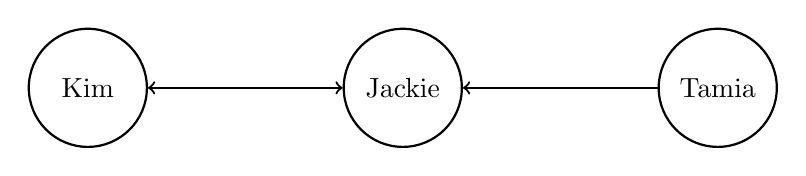
\begin{tikzpicture}[node distance={4cm}, thick, main/.style = {draw, circle},minimum size=1.5cm]
\node[main] (1) {Kim}; 
\node[main] (2) [right of=1] {Jackie}; 
\node[main] (3) [right of=2] {Tamia}; 

\draw[<->] (1) -- (2);  
\draw[->] (3) -- (2); 
\end{tikzpicture}
\end{center}

Given our language, we can then express simple things like:
\begin{gather}
 \exists x \exists y L(x, y)\\
 \exists x \forall y L(x, y)\\
 \forall x \exists yL(x,y)\\
 \forall x \forall y L(x, y)
\end{gather}
And as it turns out, all of these mean completely different things! In order to see this, however, we need to see how to go on calculating, once we passed one quantifier, and moved to another. 

\subsection{Existential-existential}

In the simplest case, we have $\exists x \exists y L(x,y)$. This may be read as ``There is an $x$ and a $y$ such that $x$ loves $y$'', or in other words, there is at least one pair of people such that one loves the other. 

As usual, the question is whether $\exists x \exists y L(x, y)$ is true in $\mathbf{S}$ or not. That is, is it the case that $\mathbf{S} \models \exists x \exists y L(x, y)$? By the above, we know that this should come out true, but how? 

The reasoning is a simple generalization of the previous one. Previously, for atomic formulas with a unary predicate, we had: 

\begin{quote}
	$\mathbf{S} \models \exists x P(x)[\mathbf{a}]$ \textit{iff} there is an $x$-variant assignment $\mathbf{a}'$ such that $\mathbf{S} \models P(x)[\mathbf{a}']$. 
\end{quote}
%
We can generalize this to \textit{any} formula $Y$ of $\mathcal{L}_1$ so that it says:
%
\begin{quote}
	$\mathbf{S} \models \exists x Y[\mathbf{a}]$ \textit{iff} there is an $x$-variant assignment $\mathbf{a}'$ such that $\mathbf{S} \models Y[\mathbf{a}']$. 
\end{quote}

Note that $Y$ here may be \textit{any} formula whatsoever, including one that already has quantifiers in it. This allows us to calculate our way through multiple quantifiers in a formula. 

\fpbox{As we discussed before, semantic rules for formulas are always formulated in parallel to the syntactic rules. Since we have a syntactic rule that says for any formula $Y$, you can put $\exists x$  ($\forall x$) in front to get a quantified formula $\exists x Y$ ($\forall x Y$), we needed a semantic rule in just those terms. The above is exactly that, in terms of the existential quantifier. Thus, once more, our semantic calculations will stepwise follow the steps of the syntactic breakdown of any formula.}

Let's return to our sentence $\exists x \exists y L(x, y)$. As mentioned, this should come out true. Let's see how this comes about using our definitions. First, take any $\mathbf{a}$ whatsoever, since this is a sentence. Then, let's see when it is the case that $\mathbf{S} \models \exists x \exists y L(x, y)[\mathbf{a}]$. Well, by the above, we have that:

\begin{quote}
	$\mathbf{S} \models \exists x \exists y L(x,y)[\mathbf{a}]$ \textit{iff} there is an $x$-variant assignment $\mathbf{a}'$ such that $\mathbf{S} \models \exists y L(x,y)[\mathbf{a}']$. 
\end{quote}

Note that we got rid of the first quantifier. However, we are now working with a hypothesis, choosing a value for $x$ that we think will make the resulting formula $\exists yL(x,y)$ satisfied under $\mathbf{a}'$ (and not $\mathbf{a}$ anymore). Since we see the definition of $I$ as regards $L$, we know that Jackie and Kim is a good pair to choose, since by $I(L)$, they love each other (and specifically, Jackie loves Kim). So let's choose the $x$-variant assignment $\mathbf{a}^x_\text{Jackie}$. Then, we need to plug these new values into the definition to calculate again. In particular:

\begin{quote}
	$\mathbf{S} \models \exists y L(x,y)[\mathbf{a}^x_\text{Jackie}]$ \textit{iff} there is a $y$-variant (!) assignment $(\mathbf{a}^x_\text{Jackie})'$ such that $\mathbf{S} \models L(x,y)[(\mathbf{a}^x_\text{Jackie})']$. 
\end{quote}

Again, the hypothesis is that if $x$ evaluates to Jackie, then we should find a value for $y$ such that $L(x, y)$ becomes satisfied in $\mathbf{S}$. Of course, this happens precisely when $y$ evaluates to Kim. So we take the $y$-variant assignment of $\mathbf{a}^x_\text{Jackie}$ (and not $\mathbf{a}$!) that still assigns Jackie to $x$, but now also explicitly assigns Kim to $y$. We can represent this as $(\mathbf{a}^x_\text{Jackie})^y_\text{Kim}$. This is the assignment that is just like $\mathbf{a}$ except $x$ is assigned Jackie, and $y$ is assigned Kim. Thus, we have that: 
\[
\mathbf{S}\models L(x, y)[(\mathbf{a}^x_\text{Jackie})^y_\text{Kim}].
\]

Since there are no more quantifiers to deal with, and there were no connectives to begin with, this is where we bottom out. Thus, it is shown that $\mathbf{S} \models \exists x \exists y L(x, y)[\mathbf{a}]$.

Here are the steps again, in succession:
%
\begin{align*}
\mathbf{S} \models & \exists x \exists y L(x, y)[\mathbf{a}]\\
\mathbf{S} \models & \exists y L(x,y)[\mathbf{a}^x_\text{Jackie}]\\
\mathbf{S}\models & L(x, y)[(\mathbf{a}^x_\text{Jackie})^y_\text{Kim}].
\end{align*}
%
Again, as you can see, we are working parallel to the syntactic analysis of the formula, namely, taking off a quantifier at each turn until we get to the atomic formula. And semantically, what we are trying to make sure at each turn is to have the final (now open) formula satisfied under the new assignment we constructed. 

Thinking in terms of mathematics, you may think of this as finding a solution to the final expression $L(x, y)$ by finding an appropriate value for $x$, and for $y$, that makes $L(x, y)$ come out correct. And thinking intuitively, we just found two people in the domain of the structure such that one loves the other, and derived that the sentence ``There are two people such that one loves the other'' is therefore true relative to the structure. 

\subsection{Existential-universal}

When it comes to the use of the universal quantifier, things get more interesting. In the case of the existential quantifier, we only had to look at single solutions. But when it comes to the universal quantifier, we have to check whether everything is a solution. Again, we can generalize the previous definition for the universal to cover every formula as such:

\begin{quote}
	$\mathbf{S} \models \forall x Y[\mathbf{a}]$ \textit{iff} for every $x$-variant assignment $\mathbf{a}'$, $\mathbf{S} \models Y[\mathbf{a}']$. 
\end{quote}

As you can see, this says that $\forall x Y$ is satisfied in $\mathbf{S}$ relative to $\mathbf{a}$ \textit{iff} \textit{every} $x$-variant assignment $\mathbf{a}'$ satisfies $Y$ in $\mathbf{S}$. This gets more complicated when we examine how this relates to the other quantifiers in a certain formula. Of course, in general, the calculation steps are always given by the definitions, but carrying them out correctly is crucial. 

Let's take the next formula, then, $\exists x \forall y L(x, y)$. Using our usual gloss, this means that there is \textit{someone} in our domain such that they love \textit{everyone}. Thus, if we are trying to figure out whether this is true or false, we need to consider every person, and see whether any of them is such that they love everyone. As it turns out, this is \textit{false}. In fact, you have to be careful here, since loving \textit{everyone} would mean that they love \textit{themselves} too! By that fact alone, there is no one in the domain that loves everyone. Why is this case?

Well, again, we add an arbitrary assignment $\mathbf{a}$ to start with, and get to the instance of the $\exists$-definition:

\begin{quote}
	$\mathbf{S} \models \exists x \forall y L(x,y)[\mathbf{a}]$ \textit{iff} there is an $x$-variant assignment $\mathbf{a}'$ such that $\mathbf{S} \models \forall y L(x,y)[\mathbf{a}']$. 
\end{quote}

Thus, we need to find a value for $x$ that would make the open formula $\forall y L(x, y)$ satisfied in the structure $\mathbf{S}$, which in turn would mean the open formula $L(x, y)$ satisfied for \textit{every} value of $y$ in turn. Since this is a finite structure, this can be checked mechanically, by taking each value one by one. 

In particular, any possible solution would need to assign a value to $x$ to start. Plugging these into our $\forall$-definition, we have that: 

\begin{enumerate}
\item	$\mathbf{S} \models \forall y L(x,y)[\mathbf{a}^x_\text{Jackie}]$ \textit{iff} for every $y$-variant assignment $(\mathbf{a}^x_\text{Jackie})'$, $\mathbf{S} \models L(x,y)[(\mathbf{a}^x_\text{Jackie})']$;
\item $\mathbf{S} \models \forall y L(x,y)[\mathbf{a}^x_\text{Kim}]$ \textit{iff} for every $y$-variant assignment $(\mathbf{a}^x_\text{Kim})'$, $\mathbf{S} \models L(x,y)[(\mathbf{a}^x_\text{Kim})']$;
\item $\mathbf{S} \models \forall y L(x,y)[\mathbf{a}^x_\text{Tamia}]$ \textit{iff} for every $y$-variant assignment $(\mathbf{a}^x_\text{Tamia})'$, $\mathbf{S} \models L(x,y)[(\mathbf{a}^x_\text{Tamia})']$.
\end{enumerate}

The next question is if we can make the right hand side of \textit{any} of these true. And the answer, again, is no. To each of these, there is a counterexample. In particular, each counterexample shows that for every choice of $x$, we can find a value for $y$ such that $x$ does \textit{not} love $y$, thereby making sure that there is no one that loves everyone. 

In particular, we have that:

\begin{enumerate}
	\item $\mathbf{S} \not\models L(x,y)[(\mathbf{a}^x_\text{Jackie})^y_\text{Jackie}]$;
	\item $\mathbf{S} \not\models L(x,y)[(\mathbf{a}^x_\text{Kim})^y_\text{Kim}]$;
	\item $\mathbf{S} \not\models L(x,y)[(\mathbf{a}^x_\text{Tamia})^y_\text{Tamia}]$.
\end{enumerate}

In other words, Jackie dos not love Jackie, Kim does not love Kim, Tamia does not love Tamia, and therefore, there is no one that loves everyone. So we can conclude that:
\[
\mathbf{S} \not\models \exists x \forall y L(x, y).
\]

Before moving forward, we should note that the above way of checking the truth of a quantified sentence is not always possible, since some structures are infinite. For example, if $\mathbf{S}'=\oset{\mathbb{N}, I}$, where $I(L)=\set{\oset{j, k} \mid j\leq k}$, then it is true that $\exists x \forall y L(x, y)$. That is, there is a particular natural number that is less than or equal to \textit{every} other natural number. That number is $0$. The problem is that the relevant instance of this is: 

\begin{quote}
	$\mathbf{S} \models \forall y L(x,y)[\mathbf{a}^x_0]$ \textit{iff} for every $y$-variant assignment $(\mathbf{a}^x_0)'$, $\mathbf{S} \models L(x,y)[(\mathbf{a}^x_0)']$
\end{quote}

The above is clearly true, since $0$ is less than or equal to every number (including itself!). But you cannot \textit{mechanically} check this for \textit{every} number one by one, since there are infinitely many of them! Thankfully, mathematicians have ways of proving facts about infinitely many things that do not require an infinite amount of time to carry out. We shall not go into this, and freely refer to facts like $0$ is less than or equal to every other number. 

\subsection{Universal-existential}

Now let's consider the formula $\forall x \exists y L(x, y)$. Does this mean the same thing as $\exists x \forall y L(x,y)$? In fact, it does not! Note that one says that there is an $x$ which is in the relation $L$ for \textit{every} $y$, and the other one says every $x$ is in the relation $L$ with \textit{some} $y$. These two are not, in general, equivalent. For example, if we read $L$ as `loves', $\exists x \forall y L(x,y)$ says, as we have just seen, that there is someone who loves everyone. On the other hand, if we take $\forall x \exists y L(x, y)$, this says that everyone loves someone. In fact, if we check the second sentence, unlike the first, it will come out \textit{true} in $\mathbf{S}$!

Here, we start with the $\forall$-definition, since the first quantifier is a universal. Thus:
%
\begin{quote}
	$\mathbf{S} \models \forall x \exists y L(x,y)[\mathbf{a}]$ \textit{iff} for every $x$-variant assignment $\mathbf{a}'$, $\mathbf{S} \models \exists y L(x,y)[\mathbf{a}']$. 
\end{quote}
%
Again, we need to continue with the right hand side. In particular, we need to check whether for every choice of value for $x$, there is a choice of $y$ for which $L(x,y)$ is satisfiable in $\mathbf{S}$.

We only have three people in our domain, so checking for every value of $x$ is not a \textit{huge} pain. In particular, we need to check each of: 

\begin{enumerate}
	\item	$\mathbf{S} \models \exists y L(x,y)[\mathbf{a}^x_\text{Jackie}]$ \textit{iff} there is a $y$-variant assignment $(\mathbf{a}^x_\text{Jackie})'$ such that $\mathbf{S} \models L(x,y)[(\mathbf{a}^x_\text{Jackie})']$;
	\item $\mathbf{S} \models \exists y L(x,y)[\mathbf{a}^x_\text{Kim}]$ \textit{iff} there is a $y$-variant assignment $(\mathbf{a}^x_\text{Kim})'$ such that $\mathbf{S} \models L(x,y)[(\mathbf{a}^x_\text{Kim})']$;
	\item $\mathbf{S} \models \exists y L(x,y)[\mathbf{a}^x_\text{Tamia}]$ \textit{iff} there is a $y$-variant assignment $(\mathbf{a}^x_\text{Tamia})'$ such that $\mathbf{S} \models L(x,y)[(\mathbf{a}^x_\text{Tamia})']$.
\end{enumerate}

Notice that unlike before, we want each of the right hand sides to hold, since we need to consider \textit{every} possible value for $x$ in the domain. On the other hand, for each of the three, we only need to find a single value for $y$ for which $L(x, y)$ is satisfied. This can be done easily: 

\begin{enumerate}
	\item $\mathbf{S} \models L(x,y)[(\mathbf{a}^x_\text{Jackie})^y_\text{Kim}]$;
	\item $\mathbf{S} \models L(x,y)[(\mathbf{a}^x_\text{Kim})^y_\text{Jackie}]$;
	\item $\mathbf{S} \models L(x,y)[(\mathbf{a}^x_\text{Tamia})^y_\text{Jackie}]$.
\end{enumerate}

Thus, for \textit{every} choice of $x$, there is a choice for $y$ such that $L(x, y)$ is satisfied in $\mathbf{S}$. So as expected: 
\[
\mathbf{S} \models \forall x \exists y L(x, y).
\]

\subsection{Universal-universal}

If we take our calculations stepwise, it is the formula $\forall x \forall y L(x, y)$ that will take the most amount of time, since we need to check $L(x, y)$ in $\mathbf{S}$ for \textit{every} pair of values $x$ and $y$. Since we have three people in our domain, this will mean checking $L(x, y)$ for 9 pairs of values (an exponential growth!). For what the sentence $\forall x \forall y L(x, y)$ says relative to $\mathbf{S}$ is that \textit{everyone} loves \textit{everyone}. This means that for each person, we have to check that person's relation to every other person. 

Of course, as you may see, this sentence is \textit{false} in $\mathbf{S}$. In fact, for every person, there are two people whom they do not love. Kim does not love Tamia, Jackie does not love Tamia, and Tamia does not love Kim, and nobody loves themselves. Any one of these is sufficient to conclude that not everyone loves everyone. But if we want to check it directly, we need to consider all 9 $y$-variant-of-the-$x$-variant-of-$\mathbf{a}$. We can represent all these assignments in three subsequent graphs for each choice of $x$, to make it more vivid. Thus:

\begin{center}
\begin{tabular}{cc}
\begin{forest}
			[$\mathbf{a}^x_\text{Jackie}$
				[$(\mathbf{a}^x_\text{Jackie})^y_\text{Jackie}$]
				[$(\mathbf{a}^x_\text{Jackie})^y_\text{Kim}$]
				[$(\mathbf{a}^x_\text{Jackie})^y_\text{Tamia}$]
	]
\end{forest}
&
\begin{forest}
			[$\mathbf{a}^x_\text{Kim}$
[$(\mathbf{a}^x_\text{Kim})^y_\text{Kim}$]
[$(\mathbf{a}^x_\text{Kim})^y_\text{Jackie}$]
[$(\mathbf{a}^x_\text{Kim})^y_\text{Tamia}$]
]
\end{forest}
\end{tabular}
\begin{forest}
			[$\mathbf{a}^x_\text{Tamia}$
[$(\mathbf{a}^x_\text{Tamia})^y_\text{Tamia}$]
[$(\mathbf{a}^x_\text{Tamia})^y_\text{Jackie}$]
[$(\mathbf{a}^x_\text{Tamia})^y_\text{Kim}$]
]
\end{forest}
\end{center}

Again, as mentioned above, relative to any of the 9 leaves in the above trees, $L(x, y)$ should come out satisfied in $\mathcal{L}_1$. So there are 6 assignments, 2 for each tree, that entail individually that 
\[\mathbf{S}\not\models\forall x \forall y L(x, y).\]

\section{Putting it all together}

Using the above techniques, one can calculate the truth-value of any sentence in $\mathcal{L}_1$, involving any number of quantifiers in any possible distribution. And in fact, one can also calculate the satisfaction of every formula of $\mathcal{L}_1$ relative to an initial assignment $\mathbf{a}$ in the structure $\mathbf{S}$, involving open formulas with quantifiers. At each step, one just has to apply the relevant definition for the quantifier or connective until none are left, and then calculate the satisfiability of each resulting atomic formula relative to the relevant assignments. As we shall see soon, there are various techniques that make this easier than it first appears. But first, let's formulate the semantics for our language $\mathcal{L}_1$ as a whole. 

Again, the semantics is \textit{compositional}, where the meaning of more complex expressions will always be calculable from the meaning of their constituent parts. Thus, parallel to how we introduced the semantics above, our definition will also start with assigning meaning to the predicates and terms of the language, then to atomic formulas, and then to more complex formulas. 

Returning to satisfaction and truth once more, truth will be defined as a special case of satisfaction. Namely, satisfaction is relativized to structures and variable assignments, while truth will be assigned to those formulas in a structure that are satisfied under \textit{every} possible variable assignment in the domain of that structure. In other words, only some formulas satisfiable in a structure will be said to be true, those that are satisfied under every variable assignment in the domain of the structure. 

\begin{defn}[Semantics of $\mathcal{L}_1$]
A first-order structure $\mathbf{S}$ is a pair $\oset{\mathbf{D}, I}$ where $\mathbf{D}$ is a non-empty set called the \textit{domain}, and $I$ is the \textit{interpretation function} such that for every $c \in \mathsf{CONS}_{\mathcal{L}_1}$, $I(c) \in \mathbf{D}$, and for every predicate of arity $n$, $I(P^n) \subseteq \mathbf{D}^n$.

The function $\mathbf{a}: \textsf{VAR}_{\mathcal{L}_1} \to \mathbf{D}$ is a \textit{variable assignment} in $\mathbf{D}$. If $\mathbf{a}'$ is a variable assignment in $\mathbf{D}$ just like $\mathbf{a}$, except possibly for some $x$, $\mathbf{a}'(x)\neq \mathbf{a}(x)$, we call $\mathbf{a}'$ an $x$-variant variable assignment of $\mathbf{a}$. If $\mathbf{a}'(x)=d$ ($d \in \mathbf{D}$), i.e., $\mathbf{a}'$ is the $x$-variant variable assignment of $\mathbf{a}$ such that $x$ is sent to $d$ by $\mathbf{a}'$, we may also write $\mathbf{a}^x_d$.

For each term $t \in \mathsf{TERM}_{\mathcal{L}_1}$, we define the value of $t$ in the structure $\mathbf{S}$ relative to the variable assignment $\mathbf{a}$ as follows:
\begin{enumerate}
	\item if $t=x$ for some $x \in \textsf{VAR}_{\mathcal{L}_1}$, $I(t)[\mathbf{a}]=\mathbf{a}(x)$;
	\item if $t=c$ for some $c \in \textsf{CONS}_{\mathcal{L}_1}$, $I(t)[\mathbf{a}]=I(c)$.
\end{enumerate}

We define satisfaction for a formula $X$ relative to $\mathbf{S}$ under $\mathbf{a}$, in symbols, $\mathbf{S} \models X[\mathbf{a}]$ as follows:

\begin{enumerate}
	\item For the base: if $X=P^n(t_1, ..., t_n)$, then $\mathbf{S} \models X[\mathbf{a}]$ \textit{iff} $\oset{I(t_1)[\mathbf{a}], ..., I(t_n)[\mathbf{a}]} \in I(P^n)$.
	\item For the connectives: 
		\begin{enumerate}
		\item if $X=\neg Y$, $\mathbf{S} \models X[\mathbf{a}]$ \textit{iff} $\mathbf{S} \not\models Y[\mathbf{a}]$;
		\item if $X=(Y \wedge Z)$, $\mathbf{S} \models X[\mathbf{a}]$ \textit{iff} $\mathbf{S} \models Y[\mathbf{a}]$ and $\mathbf{S}\models Z[\mathbf{a}]$;
		\item if $X=(Y \vee Z)$,  $\mathbf{S} \models X[\mathbf{a}]$ \textit{iff} $\mathbf{S} \models Y[\mathbf{a}]$ or $\mathbf{S}\models Z[\mathbf{a}]$ (or both);
		\item if $X=(Y \rightarrow Z)$,  $\mathbf{S} \models X[\mathbf{a}]$ \textit{iff} if $\mathbf{S} \models Y[\mathbf{a}]$, then $\mathbf{S}\models Z[\mathbf{a}]$.
		\end{enumerate}
	\item For the quantifiers:
		\begin{enumerate}
		\item if $X =\exists x Y$, then $\mathbf{S} \models X[\mathbf{a}]$ \textit{iff} there is an $x$-variant assignment $\mathbf{a}'$ such that $\mathbf{S} \models Y[\mathbf{a}']$;
		\item if $X =\forall x Y$, then $\mathbf{S} \models X[\mathbf{a}]$ \textit{iff} for every $x$-variant assignment $\mathbf{a}'$, $\mathbf{S} \models Y[\mathbf{a}']$.
		\end{enumerate}
\end{enumerate}

We say that a formula $X$ is \textit{true in} (or \textit{relative to}) $\mathbf{S}$ \textit{iff} for every assignment $\mathbf{a}$ (in $\mathbf{D}$ of $\mathbf{S}$), $\mathbf{S} \models X[\mathbf{a}]$. We say that a formula $X$ is \textit{false in}  (or \textit{relative to}) $\mathbf{S}$ \textit{iff} for every assignment $\mathbf{a}$ (in $\mathbf{D}$ of $\mathbf{S}$), $\mathbf{S} \not\models X[\mathbf{a}]$.
\end{defn}

\fpbox{You may see something strange with this definition of falsity. In particular, we defined a formula $X$ being false \textit{not} as it not being true, but as a separate condition (namely, being unsatisfied under every assignment in $\mathbf{S}$). The reason why this is the case is precisely because some formulas cannot be said to be true or false, as they depend on the assignment function for their evaluation. Accordingly, if we specified that the formulas that are not true are false, we would have had to deem false those formulas that are sometimes satisfied, sometimes aren't in $\mathbf{S}$. It should be noted however that as far as sentences are concerned, a sentence not being true \textit{does} entail it being false, so we are not violating the Law of Excluded Middle.}

\section{The full force of the semantics}

Now that we have everything in place, we can start appreciating how expressive our language $\mathcal{L}_1$ is. So far, in our examples, we only considered ourselves with complex formulas without quantifiers, and with multiple quantifiers in front of an atomic formula, with some negations thrown in here and there. But of course, the real magic happens when we use the quantifiers and the connectives together to form complex sentences. 

To make this more vivid, we may consider a possible real life application; a webshop's database of items. The website sells clothing items in the following categories: shoes, bottoms, tops, and accessories. Moreover, each item has one or more associated color (black, white, red, green, blue), and one or more associated material (cotton, polyester, polycotton, leather). All in all, the database has information about 10 pieces of clothing items. These, we can refer to by their associated `code': $1$, $2$, $3$, and so on. 

All of this we can formally represent in a first-order structure. To make the particulars more easily readable, we will represent them in a table as follows:

\begin{center}
\begin{tabular}{l|l|l|l}
\textbf{Item} & \textbf{Category} & \textbf{Color(s)} & \textbf{Fabric}\\\hline\hline
$1$ & top& red, green & cotton \\ \hline
$2$ & top& white & cotton \\ \hline
$3$ &top& red, blue & cotton \\\hline
$4$ & top& blue & cotton \\\hline
$5$ & bottom & green & cotton \\ \hline
$6$ & bottom & red, white & polycotton \\ \hline
$7$ & shoes& white & polyester, cotton \\\hline
$8$ & shoes& blue & polyester, cotton \\\hline 
$9$ & shoes& white &   polyester, cotton \\\hline
$10$ & accessory & blue, white & polyester, cotton  
\end{tabular}
\end{center}

Then, we can use the following predicates, with their interpretation specified relative to the table above:

\begin{enumerate}
	\item Category predicates:
	\begin{enumerate}
	\item $I(Top)=\{x \mid x\text{ is a top}\}$
	\item $I(Bot)=\{x \mid x\text{ is a bottom}\}$
	\item $I(Sho)=\{x \mid x\text{ is a pair of shoes}\}$
	\item $I(Acc)=\{x \mid x\text{ is an accessory}\}$
	\end{enumerate}
	\item Color predicates:
	\begin{enumerate}
	\item $I(Red)=\{x \mid x\text{ is red}\}$
	\item $I(Gre)=\{x \mid x\text{ is green}\}$
	\item $I(Blu)=\{x \mid x\text{ is blue}\}$
	\item $I(Whi)=\{x \mid x\text{ is white}\}$
	\item $I(Bla)=\{x \mid x\text{ is black}\}$
	\end{enumerate}
	\item Fabric predicates:
	\begin{enumerate}
	\item $I(Cot)=\{x \mid x\text{ is made of cotton}\}$
	\item $I(Pol)=\{x \mid x\text{ is made of polyester}\}$
	\item $I(Pc)=\{x \mid x\text{ is made of polycotton}\}$
	\item $I(Lea)=\{x \mid x\text{ is made of leather}\}$
	\end{enumerate}
\end{enumerate}

\fpboxstar{Here is an interesting fabric fact. Some items are made out of polycotton, while some items are made out of polyester \textit{and} cotton. We can distinguish between these two as follows. Polycotton is a fabric blend that is made out of both polyester \textit{and} cotton. For example, many t-shirts are made entirely out of polycotton. But there are also some items that are made of pure cotton and pure polyester in some way combined. For example, you might buy some cotton shoes that have a polyester brand label. This does not make the shoes polycotton.}

Let's call the structure determined by the above information $\mathbf{W}$ (for a change). Once $\mathbf{W}$ is fixed, we can try and express a number of complex facts about $\mathbf{W}$, and in particular, about the various relations between these items and their properties. 

\subsection{Quantifier placement}

Let's start with some simple facts. First, you might want to express something like the following: ``There is a red top and a white top''. You might hesitate between the following two options: 
\begin{gather*}
	\exists x ((Red (x) \wedge Top(x)) \wedge (Whi(x) \wedge Top(x)))\\
	\exists x (Red(x) \wedge Top(x)) \wedge \exists x (Whi(x) \wedge Top(x))
\end{gather*}
In such cases, the correct option is the second one. For note that what the first option says is that there is a red and white top (that is a top). You can easily see this if you do the calculations explicitly, for in the first case, we need to find a single $x$-variant assignment that would satisfy the formula $((Red (x) \wedge Top(x)) \wedge (Whi(x) \wedge Top(x)))$. This is clearly impossible, for there is no one item that is a top, and both red and white. In the second case, however, we consider the two conjuncts separately, and thus we \textit{can} consider two distinct $x$-variant assignments (two distinct objects). Accordingly, in $\mathbf{W}$, the first sentence is false, while the second is true. We can see how the second sentence is true in $\mathbf{W}$ as follows:

\begin{center}
\begin{forest}
	[{$\mathbf{W} \models \exists x (Red(x) \wedge Top(x)) \wedge \exists x (Whi(x) \wedge Top(x))[\mathbf{a}]$}
		[{$\mathbf{W} \models \exists x (Red(x) \wedge Top(x)) [\mathbf{a}]$}
			[{$\mathbf{W} \models Red(x) \wedge Top(x) [\mathbf{a}^x_1]$}
				[{$\mathbf{W} \models Red(x) [\mathbf{a}^x_1]$}]
				[{$\mathbf{W} \models Top(x) [\mathbf{a}^x_1]$}]
			]
		]
		[{$\mathbf{W} \models \exists x (Whi(x) \wedge Top(x)) [\mathbf{a}]$}
			[{$\mathbf{W} \models Whi(x) \wedge Top(x) [\mathbf{a}^x_2]$}
				[{$\mathbf{W} \models Whi(x) [\mathbf{a}^x_2]$}]
				[{$\mathbf{W} \models Top(x) [\mathbf{a}^x_2]$}]
			]
		]
	]
\end{forest}
\end{center}

A similar problem arises if, for example, we change the conjunction to a disjunction, and the existential quantifier to a universal one. Suppose we want to express the fact that every item in the database is either made (at least partly) of polycotton, or made (at least partly) of cotton. Again, you have two options: 
\begin{gather*}
	\forall x (Pc(x) \vee Cot(x))\\
	\forall x Pc(x) \vee \forall x Cot(x)
\end{gather*}

Now the first sentence is the correct choice, and the second is the incorrect one. For note that what the second sentence says is really that either everything is made of polycotton, or everything is made of cotton. This sentence is a disjunction, so it is true if one of the disjuncts is true. But taken separately, it is \textit{not} true that everything is made of polycotton, and it is also not true that everything is made of cotton. In particular, we can refer to the fact that $1$ is not made of polycotton, while $6$ is not made of cotton. Thus:

\begin{center}
\begin{forest}
	[{$\mathbf{W}\not\models\forall x Pc(x) \vee \forall x Cot(x)[\mathbf{a}]$}
		[{$\mathbf{W}\not\models\forall x Pc(x) [\mathbf{a}]$}
			[{$\mathbf{W}\not\models Pc(x) [\mathbf{a}^x_1]$}]
		]
		[{$\mathbf{W}\not\models \forall x Cot(x)[\mathbf{a}]$}
			[{$\mathbf{W}\not\models Cot(x)[\mathbf{a}^x_6]$}]
		]
	]
\end{forest}
\end{center}

But again, we do have that $\mathbf{S} \models \forall x(Pc(x) \vee Cot(x))$, since for every $x$-variant assignment $\mathbf{a}'$, we have that $\mathbf{S} \models Pc(x) \vee Cot(x)[\mathbf{a}']$.

\subsection{Restricted quantification}

Let's try and formulate some more interesting facts about our database. For example, we might want to capture some interrelations between various properties of our objects. One such fact would be the following: ``If something is blue, then it is made of cotton''. 

The first question here would be: which quantifier are we supposed to use? From the above formulation, this is not clear, and indeed, the use of `something' might be misleading. Suppose you went with:
\[
\exists x (Blu(x) \rightarrow Cot(x))
\]
This sentence is true in $\mathbf{W}$ if there is a value for $x$ relative to which $Blu(x) \rightarrow Cot(x)$ is satisfied. There are several problems with this option. First, since this is an existentially quantified sentence, it is sufficient for a single object to satisfy $Blu(x) \rightarrow Cot(x)$ for the sentence to be true. This does not seem like what we are trying to express, which is a general rule applying to \textit{every} thing that is blue. 

But there is another misleading element here: the use of a conditional after an existential quantifier. As mentioned several times already, a conditional is \textit{only} unsatisfied (false) if its antecedent is satisfied (true), but its consequent is unsatisfied (false). In this case, this means that for any value for $x$, $Blu(x) \rightarrow Cot(x)$ is satisfied relative to that value provided either $Blu(x)$ and $Cot(x)$ are both satisfied, or $Blu(x)$ is \textit{not} satisfied (regardless of whether $Cot(x)$ is satisfied or not). This means that item $6$ being red, white, and polycotton is by itself sufficient to make $\exists x (Blu(x) \rightarrow Cot(x))$ true in $\mathbf{W}$, for it is \textit{not} made of cotton. This is usually not something we want to express. In general, if we wanted to express the fact that there is something that is blue and is made of cotton, then we can just say: $\exists x(Blu(x) \wedge Cot(x))$. 

Returning to our initial fact under consideration, it was \textit{not} that there is something that is blue and cotton, it was that whenever something is blue, then it is made of cotton. The correct way to capture this fact is with a universal quantifier. In particular:
\[
\forall x(Blu(x) \rightarrow Cot(x))
\]
Interestingly, once we change the quantifier to a universal one, the use of a conditional proceeding it will capture precisely what we wanted to express. In particular, the only fact that would make this sentence \textit{false} is if there were a blue item that was \textit{not} cotton. In other words, as long as there is no item that is both blue and not cotton, the sentence is true, which seems to be what we wanted to express. 

Let's choose a blue and a non-blue item from the domain, and see how this functions. First, take item number $4$, which is blue. Then, we have that:
\begin{align*}
	\mathbf{W} \models& Blu(x)[\mathbf{a}^x_4]\\
	\mathbf{W} \models& Cot(x)[\mathbf{a}^x_4]\\
	\mathbf{W} \models& Cot \rightarrow Blu(x)[\mathbf{a}^x_4]
\end{align*}
But now taking item number $5$, which is not blue, we can reason, based on the definition of satisfaction as it relates to $\rightarrow$, that:
\begin{align*}
	\mathbf{W} \not\models& Blu(x)[\mathbf{a}^x_5]\\
	\mathbf{W} \models& Cot(x)[\mathbf{a}^x_5]\\
	\mathbf{W} \models& Cot \rightarrow Blu(x)[\mathbf{a}^x_5]
\end{align*}
Naturally, we would need to check whether $Blu(x) \rightarrow Cot(x)$ is satisfied in $\mathbf{W}$ relative to every possible $x$-variant assignment, not just these two. But it is easy to see that this will indeed hold, for again, every blue thing is cotton, and the non-blue things cannot make the sentence false. 

If we zoom out for a bit, we can say that in sentences like $\forall x(Blu(x) \rightarrow Cot(x))$, the universal quantifier is \textit{restricted}. What it is restricted to is the set of things satisfying the antecedent of the conditional. For in general, the universal quantifier `ranges over' the whole domain. For example, if we had $\forall x Cot(x)$, the truth of this sentence depends on \textit{every} possible assignment of value to $x$, so every object in the domain is relevant here. On the other hand, as mentioned, once we put $Blu(x)$ in front with a conditional, we are no longer concerned with the whole domain. Rather, we \textit{restrict} our attention to just the blue things in the domain, and we say \textit{of them} that each must be cotton. Once quantification is restricted, any member of the domain not captured by the antecedent condition becomes irrelevant. 

As a rule, the universal quantification of $Z$, $\forall x Z$ is thus restricted (w.r.t. $Y$) with a conditional in the form $\forall x(Y \rightarrow Z)$. We can also talk about restricting the existential quantification of $Z$, $\exists x Z$ (w.r.t. $Y$), which is done with a conjunction (as mentioned briefly above), in the form $\exists x(Y \wedge Z)$.

\fpbox{
One problematic aspect of this is \textit{vacuous quantification}. Note that it may be the case that \textit{nothing} satisfies the antecedent of the conditional after the universal quantifier. As demonstrated above, if something does not satisfy the antecedent of the conditional, the conditional as a whole is automatically satisfied. Unfortunately, this entails that if \textit{nothing} satisfies the antecedent of the conditional, then relative to each value of $x$, the conditional as a whole is satisfied. So its universal quantification is true. For example, $\mathbf{W} \models \forall x ((Gre(x) \wedge Sho(x)) \rightarrow (Blu(x) \wedge \neg Blu(x)))$, for the sole (pun unintended) reason that there are no green shoes.
}

\subsection{Quantifying into multiple positions}

Finally, let's add even more complexity by introducing a two-place predicate $Col$, defined such that:
\[I(Col)=\set{\oset{x, y}, \mid x\text{ is part of the same collection as } y}.\]
Let's further specify that in our structure $\mathbf{W}$, there are four collections:
\begin{enumerate}
	\item Collection 1: items $2$, $6$, and $9$
	\item Collection 2: items $4$, $7$ and $10$
	\item Collection 3: items $1$, $3$, and $8$ 
	\item Collection 4: item $5$
\end{enumerate}
%
We can represent these collections in terms of the relation $I(Col)$ as in Figure \ref{partit}. As you can see, the relation allows us to separate the domain into 4 distinct, non-overlapping subsets, one for each collection, based on how the relation $I(Col)$ is distributed between the members (as represented by the arrows). The basic idea is that for any two members of the \textit{same} collection, $I(Col)$ holds, while for any two items in \textit{distinct} collections, they are never related in terms of $I(Col)$.

\begin{figure}[h]
\begin{center}
	\begin{tikzpicture}[node distance={2cm}, thick, main/.style = {draw, circle},minimum size=1cm]
		\node[main] (1) {$2$}; 
		\node[main] (2) [below left of=1] {$6$}; 
		\node[main] (3) [below right of=1] {$9$}; 
		\node (a) [above left of=1] {Collection 1};
		
		\draw[<->] (1) -- (2);  
		\draw[<->] (2) -- (3);
		\draw[<->] (3) -- (1);
		
		\node[main] (4) [right=4cm of 1] {$4$}; 
		\node[main] (5) [below left of=4] {$7$}; 
		\node[main] (6) [below right of=4] {$10$}; 
		\node (b) [above right of=4] {Collection 2};
		
		\draw[<->] (4) -- (5);  
		\draw[<->] (5) -- (6);
		\draw[<->] (6) -- (4);
		
		\node[main] (7) [below=2.5cm of 1] {$1$}; 
		\node[main] (8) [below left of=7] {$3$}; 
		\node[main] (9) [below right of=7] {$8$}; 
		\node (c) [below =1.4cm of 7] {Collection 3};
		
		\draw[<->] (7) -- (8);  
		\draw[<->] (8) -- (9);
		\draw[<->] (9) -- (7);
		
		\node[main] (10) [below=3cm of 4] {$5$}; 
		\node (d) [below=.1cm of 10] {Collection 4};
		
		\foreach \x in {1, 2,...,10} {\draw [->] (\x) edge[loop above] (\x);}
	\end{tikzpicture}
\end{center}
\caption{Partitioning the domain relative to $I(Col)$}\label{partit}
\end{figure}

\fpbox{Note that as it is specified, $I(Col)$ is a reflexive, symmetric, and transitive relation. Reflexive, because everything is in the same collection as itself. Symmetric, because if $x$ is in the same collection as $y$, then $y$ is in the same collection as $x$. And transitive, because if $x$ is in the same collection as $y$, and $y$ is in the same collection as $z$, then $x$ is in the same collection as $z$. As it turns out, such relations always \textit{partition} the domain into non-overlapping subsets, like our collections above.}

We can then use multiple quantifiers to `quantify into' the two `positions' (argument places) of the binary predicate $Col$. For example, we might want to express the fact that there is an item for which it is true that if another item is in the same collection as it is, then that second item is white. Put another way, there is an item which is in a collection of white things. This can be captured as follows:
\[
\exists x \forall y(Col(x, y) \rightarrow Whi(y))
\]
How is this sentence to be evaluated relative to $\mathbf{W}$? We need to check if we can find a value for $x$, such that for any value we can find for $y$, it is satisfied that if $x$ and $y$ are in the same collection, then $y$ is white. 

Here is what's \textit{not} going to work. Suppose you choose for $x$ the value $4$. After all, \textit{other than} $4$, every member of collection 2 is white. The problem here is that we have to check \textit{every} item in the same collection as $4$, which includes $4$ itself. And $4$ is not white! So we have that:
\begin{align*}
\mathbf{W} \not\models& \forall y(Col(x, y) \rightarrow Whi(y))[\mathbf{a}^x_4]\\
\mathbf{W} \not\models& Col(x, y) \rightarrow Whi(y)[(\mathbf{a}^x_4)^y_4]\\
\mathbf{W} \models& Col(x, y)[(\mathbf{a}^x_4)^y_4]\\
\mathbf{W} \not\models& Whi(y)[(\mathbf{a}^x_4)^y_4]
\end{align*} 
(Note that we are not saying that $\mathbf{S} \not\models \exists x \forall y(Col(x, y) \rightarrow Whi(y))$, we are saying that choosing $4$ as the value for $x$ would not satisfy $\forall y(Col(x, y) \rightarrow Whi(y))$. This does not entail that the initial formula is false, and indeed, it is true, we just have to find the right value for $x$!)

On the other hand, we may choose any one item of collection 1, for there, it is guaranteed that every member of the collection will be white (including the chosen member). For example:
%
\begin{align*}
	\mathbf{W} \models& \exists x\forall y(Col(x, y) \rightarrow Whi(y))[\mathbf{a}]\\
	\mathbf{W} \models& \forall y(Col(x, y) \rightarrow Whi(y))[\mathbf{a}^x_2]\\
	\mathbf{W} \models& Col(x, y) \rightarrow Whi(y)[(\mathbf{a}^x_2)^y_2]\\
	\mathbf{W} \models& Col(x, y) \rightarrow Whi(y)[(\mathbf{a}^x_2)^y_6]\\
		\mathbf{W} \models& Col(x, y) \rightarrow Whi(y)[(\mathbf{a}^x_2)^y_9]
\end{align*} 
%
As before, these are only the relevant $y$-variant assignments that \textit{could} make a difference. In particular, if we were to send $y$ to any member other than $2$, $6$ or $9$, the conditional would immediately be satisfied by the fact that for no other assignment to $y$ do we have $Col(x, y)$ (when $x$ is sent to $2$).

\begin{exc}
From the above, it does not follow that $\mathbf{W} \models \forall x(\exists y Col(x, y) \rightarrow Whi(y))$. Nor does it follow that $\mathbf{W} \models \forall x \forall y(Col(x, y) \rightarrow Whi(y))$  Explain why these fail to be true in $\mathbf{W}$.
\end{exc}

\subsection{Translating the untranslatable}

As our final example, let's try and capture something trickier. Suppose we want to capture the fact that there is a collection with a red and a blue item in it. At first glance, it seems like you could easy express this fact by using an existential quantifier and a predicate for `is a collection'. The problem is that we have no such predicate! We have the predicate $Col$, but that predicate says not that something is a collection, but that two items are in the \textit{same} collection. There is a reason for not including a predicate for `is a collection'. For note that one-place predicates are evaluated in our semantics as subsets of our domain, and our domain does not have collections as members in it. It only has clothing items! And if you check $Col(x, y)$, it applies to clothing items, and \textit{not} the collections, for it says that two \textit{items} $x$, $y$ are in the same collection.

On the other hand, we \textit{can} capture the above fact without talking explicitly about collections, just by using the predicate $Col$. For there being a collection with a red and a blue item in it is equivalent to saying that there are two items, one red and blue, such that they are in the same collection. If this is true, then there is a collection with a red and a blue item in it. Conversely, if there is a collection with a red and a blue item in it, then there are two items, one red, one blue that are in the same collection. (For everything in this paragraph, you should remember that there may only be a single object that has both properties.)

\fpbox{First-order languages, though very expressive, are still in some respects limited. In particular, they are limited by the fact that the quantifiers only range over members of the domain, predicates only have as interpretations subsets of the domain, and so on. On the other hand, many times (though certainly not always!), there are clever ways to turn an `untranslatable' claim into a translatable one. The touchstone for these is `truth-conditional equivalence'. All this means is that the two sentences should be true (false) under the the same circumstances.}

\noindent Accordingly, we can represent the fact that there is a collection with a red and a blue item in it as:
\[
\exists x\exists y((Red(x) \wedge Blu(y)) \wedge Col(x, y))
\]
In particular, item $1$ is red, item $3$ is blue, and they are both in collection 3. So we have:

\begin{center}
\begin{forest}
	[{$\mathbf{W}\models \exists x\exists y((Red(x) \wedge Blu(y)) \wedge Col(x, y))[\mathbf{a}]$}
		[{$\mathbf{W}\models \exists y((Red(x) \wedge Blu(y)) \wedge Col(x, y))[\mathbf{a}^x_1]$}
		[{$\mathbf{W}\models (Red(x) \wedge Blu(y)) \wedge Col(x, y)[(\mathbf{a}^x_1)^y_3]$}
			[{$\mathbf{W}\models (Red(x) \wedge Blu(y)) [(\mathbf{a}^x_1)^y_3]$}
				[{$\mathbf{W}\models Red(x) [(\mathbf{a}^x_1)^y_3]$}]
				[{$\mathbf{W}\models Blu(y) [(\mathbf{a}^x_1)^y_3]$}]
			]
			[{$\mathbf{W}\models Col(x, y)[(\mathbf{a}^x_1)^y_3]$}]
		]
		]
	]
\end{forest}
\end{center}

\medskip\hrule\medskip

Now you try it!

\begin{exc}
Try and formulate in $\mathcal{L}_1$ the fact that the relation $I(Col)$ is reflexive, symmetric, and transitive. In particular:
\begin{enumerate}
	\item Every item is in the same collection as itself.
	\item For every two items, if the first is in the same collection as the second, then the second is in the same collection as the first one.
	\item For every three items, if the first is in the same collection as the second, and the second is in the same collection as the third, then the first is in the same collection as the third. 
\end{enumerate}
\end{exc}

\begin{exc}
Try to formulate in $\mathcal{L}_1$ the following facts about $\mathbf{W}$:
\begin{enumerate}
	\item If something is made of polycotton, then it is a red and white bottom. 
	\item Every green item is either a top or a bottom. 
	\item Every item is either an accessory or not blue and white. 
	\item If something is both polyester and cotton, then it is not a top. 
	\item If something is a top, then it is only made of one material. 
	
	[Hint: something being made of one material cannot be expressed directly, but you can express each possible situation in which something is made of one thing and not the other two. One of these situations must hold if something is made of a single material.]
\end{enumerate}

In each case, explain why the fact as you translated it into $\mathcal{L}_1$ is true.
\end{exc}

\begin{remark}
Here is how your answers should look like. Suppose you want to express that no item is made of leather. 

The translation of the above fact is: $\neg \exists x Lea(x)$, since we want to express that there is no $x$ such that $x$ is made of leather. Now $\mathbf{W}\models \neg \exists Lea(x)$, since $\mathbf{W} \models \neg \exists x Lea(x)[\mathbf{a}]$ \textit{iff} $\mathbf{W} \not\models \exists x Lea(x)[\mathbf{a}]$. In turn, $\mathbf{W} \not\models \exists x Lea(x)[\mathbf{a}]$ if there is \textit{no} $x$-variant assignment $\mathbf{a}'$ such that $\mathbf{W}\models Lea(x)[\mathbf{a}']$. This means that for \textit{every} $x$-variant assignment $\mathbf{a}'$, $\mathbf{W}\not\models Lea(x)[\mathbf{a}']$. But this is the case, since nothing is made of leather, that is, $I(Lea)=\emptyset$.
\end{remark}

\begin{exc}
Write four true sentences about $\mathbf{W}$ that each contain \textit{at least} 2 quantifiers and a connective. In each case, express what fact you are capturing about $\mathbf{W}$ by the formula. 
\end{exc}

